% ============================================================
% Crescent College Face Recognition & Surveillance System
% Architecture Diagram — LaTeX / TikZ
% ============================================================
% Compile with: pdflatex architecture_latex.tex
% ============================================================

\documentclass[border=15pt, tikz]{standalone}

\usepackage[utf8]{inputenc}
\usepackage[T1]{fontenc}
\usepackage{tikz}
\usetikzlibrary{shapes, arrows, positioning, fit, calc, backgrounds}

% ── Color Definitions ──
\definecolor{bgdark}{HTML}{0A0A0A}
\definecolor{layerbg}{HTML}{0F172A}
\definecolor{nodebg}{HTML}{1E1B4B}
\definecolor{nodesurv}{HTML}{111827}
\definecolor{accent}{HTML}{6366F1}
\definecolor{accentlight}{HTML}{A78BFA}
\definecolor{textprimary}{HTML}{E2E8F0}
\definecolor{textsecondary}{HTML}{94A3B8}
\definecolor{textmuted}{HTML}{64748B}
\definecolor{jsoncolor}{HTML}{6366F1}
\definecolor{httpcolor}{HTML}{22D3EE}
\definecolor{sqlcolor}{HTML}{F59E0B}
\definecolor{apicolor}{HTML}{EF4444}
\definecolor{filecolor}{HTML}{10B981}
\definecolor{survborder}{HTML}{8B5CF6}
\definecolor{storageborder}{HTML}{10B981}
\definecolor{amberborder}{HTML}{F59E0B}

% ── Arrow Styles ──
\tikzstyle{jsonarrow} = [
  ->, >=stealth, thick, jsoncolor,
  postaction={decorate}
]
\tikzstyle{httparrow} = [
  ->, >=stealth, thick, httpcolor, dashed
]
\tikzstyle{sqlarrow} = [
  ->, >=stealth, thick, sqlcolor, dashed
]
\tikzstyle{apiarrow} = [
  ->, >=stealth, thick, apicolor, dashed
]
\tikzstyle{filearrow} = [
  ->, >=stealth, thick, filecolor
]
\tikzstyle{internalarrow} = [
  ->, >=stealth, thin, survborder
]

% ── Node Styles ──
\tikzstyle{layerbox} = [
  draw=textmuted, fill=layerbg, rounded corners=6pt,
  minimum width=17cm, inner sep=10pt, thick
]
\tikzstyle{layerlabel} = [
  font=\scriptsize\bfseries\sffamily, text=textmuted,
  anchor=north west
]
\tikzstyle{component} = [
  draw=accent, fill=nodebg, rounded corners=5pt,
  minimum height=1.2cm, text=textprimary,
  font=\small\sffamily, align=center,
  thick
]
\tikzstyle{survcomponent} = [
  draw=survborder, fill=nodebg, rounded corners=4pt,
  minimum height=1.0cm, text=textprimary,
  font=\footnotesize\sffamily, align=center,
  thin
]
\tikzstyle{storagenode} = [
  draw=storageborder, fill=nodebg, rounded corners=5pt,
  minimum height=1.2cm, text=textprimary,
  font=\small\sffamily, align=center,
  thick
]
\tikzstyle{dbnode} = [
  draw=amberborder, fill=nodebg, rounded corners=5pt,
  minimum height=1.2cm, text=textprimary,
  font=\small\sffamily, align=center,
  thick
]
\tikzstyle{externalnode} = [
  draw=apicolor, fill=nodebg, rounded corners=5pt,
  minimum height=1.0cm, text=textprimary,
  font=\small\sffamily, align=center,
  thick
]
\tikzstyle{modelnode} = [
  draw=textmuted, fill=nodebg, rounded corners=5pt,
  minimum height=1.0cm, text=textprimary,
  font=\small\sffamily, align=center
]
\tikzstyle{survbox} = [
  draw=accent, fill=nodesurv, rounded corners=5pt,
  inner sep=8pt, dashed, thick
]
\tikzstyle{flowlabel} = [
  font=\tiny\ttfamily, fill=bgdark, inner sep=1.5pt
]
\tikzstyle{pycomponent} = [
  draw=accentlight, fill=nodebg, rounded corners=5pt,
  minimum height=1.2cm, text=textprimary,
  font=\small\sffamily, align=center,
  thick
]

\begin{document}
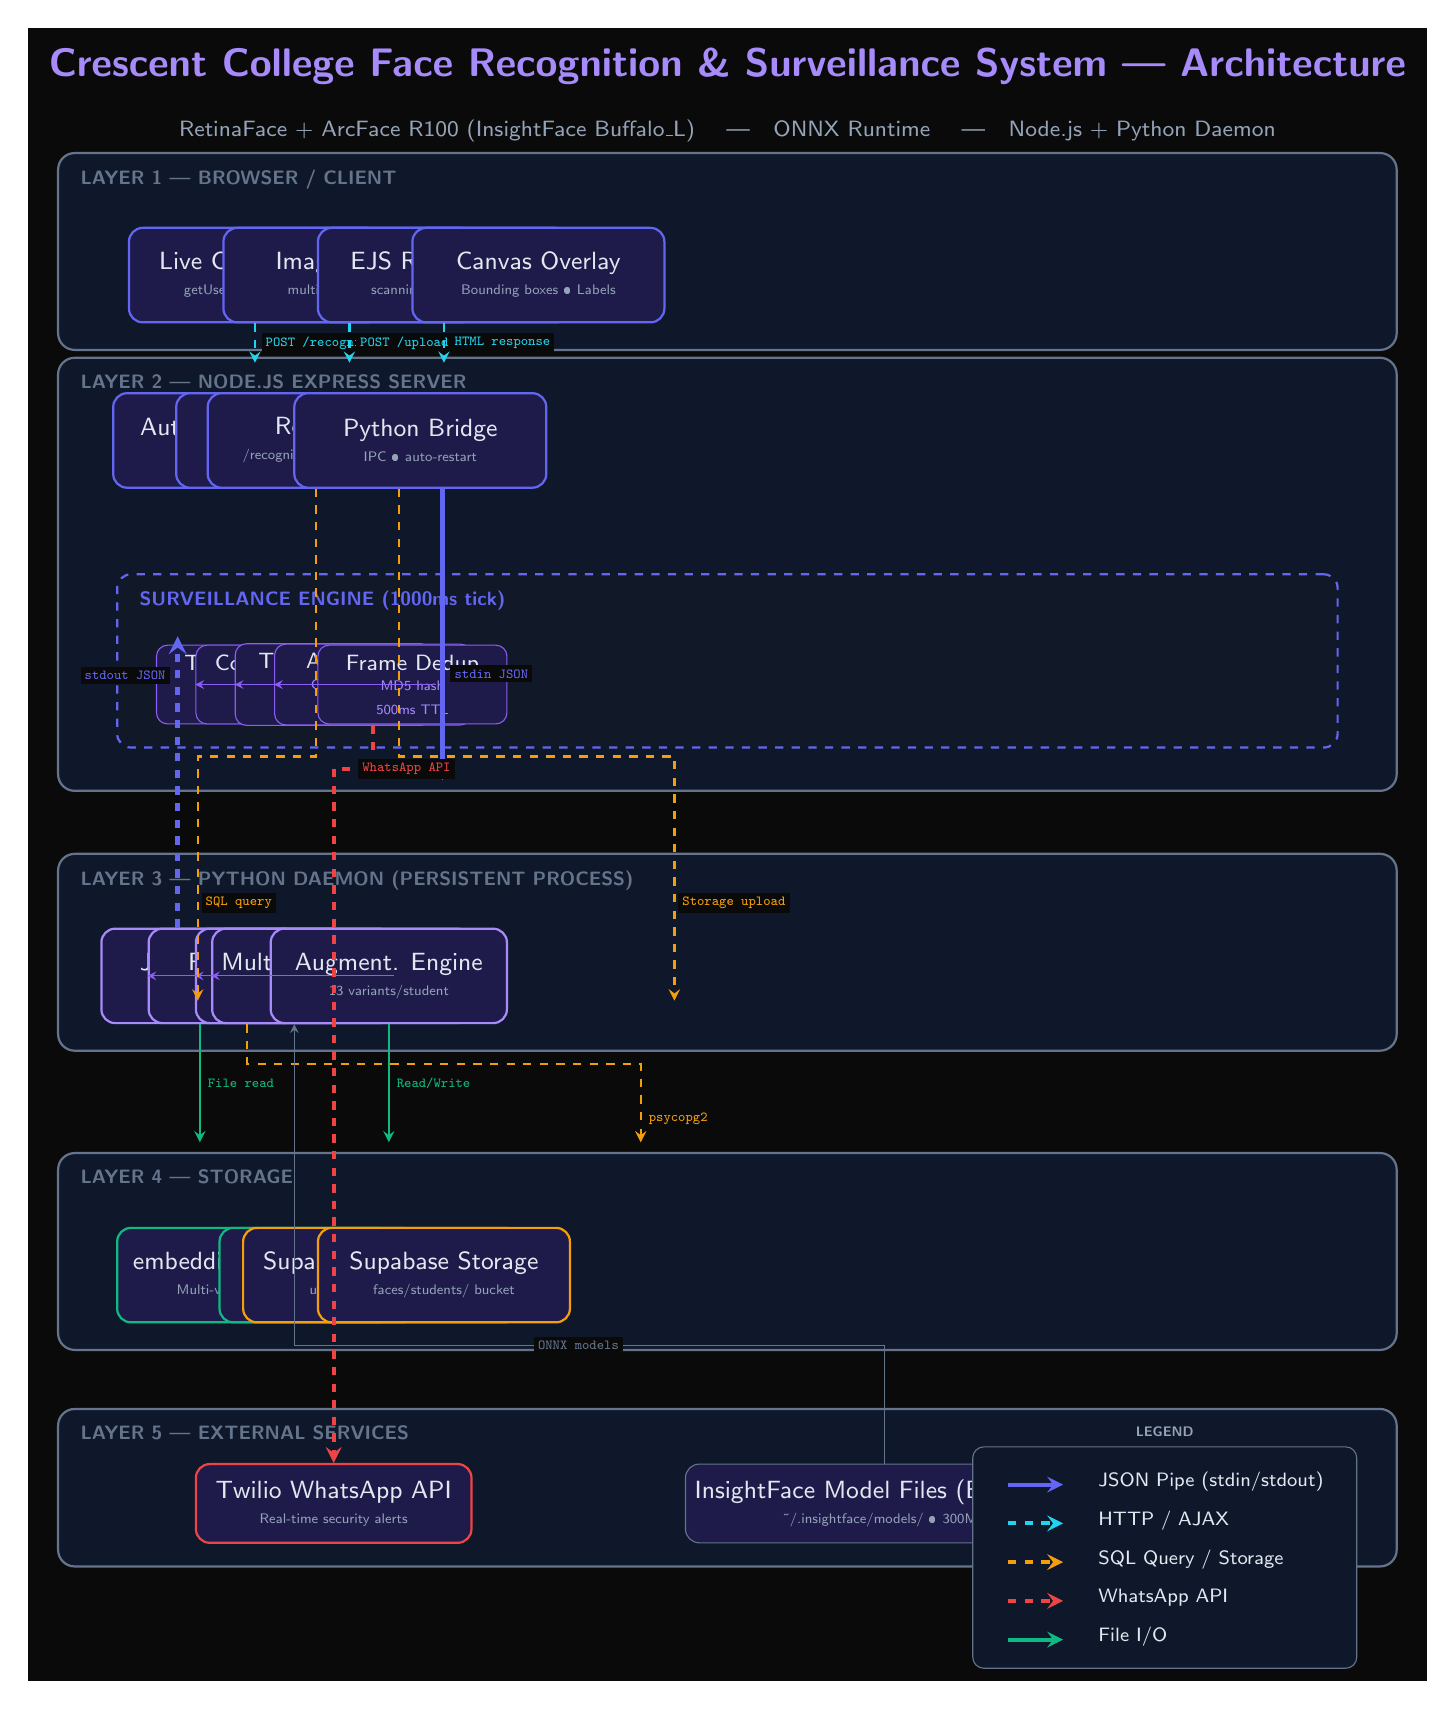
\begin{tikzpicture}[
  on grid,
  node distance=1.5cm and 1.8cm,
  background rectangle/.style={fill=bgdark},
  show background rectangle
]

% ════════════════════════════════════════════════════════════
% TITLE
% ════════════════════════════════════════════════════════════
\node[font=\Large\bfseries\sffamily, text=accentlight, anchor=south]
  (title) at (8.5, 20.5)
  {Crescent College Face Recognition \& Surveillance System --- Architecture};

\node[font=\footnotesize\sffamily, text=textsecondary, anchor=north]
  (subtitle) at (8.5, 20.3)
  {RetinaFace + ArcFace R100 (InsightFace Buffalo\_L) \quad|\quad ONNX Runtime \quad|\quad Node.js + Python Daemon};


% ════════════════════════════════════════════════════════════
% LAYER 1 — Browser / Client
% ════════════════════════════════════════════════════════════
\node[layerbox, minimum height=2.5cm] (L1) at (8.5, 18.5) {};
\node[layerlabel] at ([xshift=5pt, yshift=-3pt] L1.north west) {LAYER 1 --- BROWSER / CLIENT};

\node[component, minimum width=3.2cm] (camera)
  at (2.5, 18.2) {Live Camera Feed\\[-2pt]{\tiny\color{textsecondary} getUserMedia \textbullet{} 500ms}};

\node[component, minimum width=3.2cm, right=1.2cm of camera] (upload)
  {Image Upload\\[-2pt]{\tiny\color{textsecondary} multipart/form-data}};

\node[component, minimum width=3.2cm, right=1.2cm of upload] (ejspages)
  {EJS Result Pages\\[-2pt]{\tiny\color{textsecondary} scanning.ejs \textbullet{} result.ejs}};

\node[component, minimum width=3.2cm, right=1.2cm of ejspages] (overlay)
  {Canvas Overlay\\[-2pt]{\tiny\color{textsecondary} Bounding boxes \textbullet{} Labels}};


% ════════════════════════════════════════════════════════════
% LAYER 2 — Node.js Express Server
% ════════════════════════════════════════════════════════════
\node[layerbox, minimum height=5.5cm] (L2) at (8.5, 14.4) {};
\node[layerlabel] at ([xshift=5pt, yshift=-3pt] L2.north west) {LAYER 2 --- NODE.JS EXPRESS SERVER};

% Top row
\node[component, minimum width=3.0cm] (auth)
  at (2.2, 16.1) {Auth Middleware\\[-2pt]{\tiny\color{textsecondary} bcrypt \textbullet{} sessions}};

\node[component, minimum width=3.0cm, right=0.8cm of auth] (multer)
  {Multer Upload\\[-2pt]{\tiny\color{textsecondary} 10MB \textbullet{} images only}};

\node[component, minimum width=3.8cm, right=0.8cm of multer] (routes)
  {Route Handlers\\[-2pt]{\tiny\color{textsecondary} /recognize \textbullet{} /upload \textbullet{} /add-student}};

\node[component, minimum width=3.2cm, right=0.8cm of routes] (bridge)
  {Python Bridge\\[-2pt]{\tiny\color{textsecondary} IPC \textbullet{} auto-restart}};

% Surveillance Engine box
\node[survbox, minimum width=15.5cm, minimum height=2.2cm] (survbox)
  at (8.5, 13.3) {};
\node[layerlabel, text=accent] at ([xshift=5pt, yshift=-3pt] survbox.north west)
  {SURVEILLANCE ENGINE (1000ms tick)};

\node[survcomponent, minimum width=2.5cm] (trackMgr)
  at (2.5, 13.0) {TrackManager\\[-2pt]{\tiny\color{accentlight} Ghost tracking}\\[-1pt]{\tiny\color{accentlight} Re-identification}};

\node[survcomponent, minimum width=2.5cm, right=0.5cm of trackMgr] (confFilter)
  {ConfidenceFilter\\[-2pt]{\tiny\color{accentlight} EMA $\alpha$=0.3}\\[-1pt]{\tiny\color{accentlight} Lost @ 3 frames}};

\node[survcomponent, minimum width=2.5cm, right=0.5cm of confFilter] (threatAn)
  {ThreatAnalyzer\\[-2pt]{\tiny\color{accentlight} 4-factor scoring}\\[-1pt]{\tiny\color{accentlight} Hysteresis 5/10}};

\node[survcomponent, minimum width=2.5cm, right=0.5cm of threatAn] (alertMgr)
  {AlertManager\\[-2pt]{\tiny\color{accentlight} Cooldowns \textbullet{} Dedup}\\[-1pt]{\tiny\color{accentlight} Priority filter}};

\node[survcomponent, minimum width=2.4cm, right=0.5cm of alertMgr] (frameDedup)
  {Frame Dedup\\[-2pt]{\tiny\color{accentlight} MD5 hash}\\[-1pt]{\tiny\color{accentlight} 500ms TTL}};

% Internal arrows
\draw[internalarrow] (trackMgr.east) -- (confFilter.west);
\draw[internalarrow] (confFilter.east) -- (threatAn.west);
\draw[internalarrow] (threatAn.east) -- (alertMgr.west);


% ════════════════════════════════════════════════════════════
% LAYER 3 — Python Daemon
% ════════════════════════════════════════════════════════════
\node[layerbox, minimum height=2.5cm] (L3) at (8.5, 9.6) {};
\node[layerlabel] at ([xshift=5pt, yshift=-3pt] L3.north west) {LAYER 3 --- PYTHON DAEMON (PERSISTENT PROCESS)};

\node[pycomponent, minimum width=2.5cm] (jsonpipe)
  at (1.8, 9.3) {JSON Pipe\\[-2pt]{\tiny\color{textsecondary} stdin/stdout}};

\node[pycomponent, minimum width=2.5cm, right=0.6cm of jsonpipe] (retina)
  {RetinaFace\\[-2pt]{\tiny\color{textsecondary} det\_10g.onnx}};

\node[pycomponent, minimum width=2.5cm, right=0.6cm of retina] (arcface)
  {ArcFace R100\\[-2pt]{\tiny\color{textsecondary} w600k\_r50.onnx}};

\node[pycomponent, minimum width=3.0cm, right=0.6cm of arcface] (matcher)
  {Multi-Variant Matcher\\[-2pt]{\tiny\color{textsecondary} Cosine + eye fallback}};

\node[pycomponent, minimum width=3.0cm, right=0.6cm of matcher] (augeng)
  {Augment. Engine\\[-2pt]{\tiny\color{textsecondary} 13 variants/student}};

% Internal arrows
\draw[internalarrow] (jsonpipe.east) -- (retina.west);
\draw[internalarrow] (retina.east) -- (arcface.west);
\draw[internalarrow] (arcface.east) -- (matcher.west);


% ════════════════════════════════════════════════════════════
% LAYER 4 — Storage
% ════════════════════════════════════════════════════════════
\node[layerbox, minimum height=2.5cm] (L4) at (8.5, 5.8) {};
\node[layerlabel] at ([xshift=5pt, yshift=-3pt] L4.north west) {LAYER 4 --- STORAGE};

\node[storagenode, minimum width=3.5cm] (cache)
  at (2.5, 5.5) {embeddings\_cache.json\\[-2pt]{\tiny\color{textsecondary} Multi-variant embeddings}};

\node[storagenode, minimum width=2.5cm, right=0.8cm of cache] (imgfolder)
  {images/ folder\\[-2pt]{\tiny\color{textsecondary} Enrollment photos}};

\node[dbnode, minimum width=3.5cm, right=0.8cm of imgfolder] (supadb)
  {Supabase PostgreSQL\\[-2pt]{\tiny\color{textsecondary} users \textbullet{} students \textbullet{} logs}};

\node[dbnode, minimum width=3.2cm, right=0.8cm of supadb] (supast)
  {Supabase Storage\\[-2pt]{\tiny\color{textsecondary} faces/students/ bucket}};


% ════════════════════════════════════════════════════════════
% LAYER 5 — External Services
% ════════════════════════════════════════════════════════════
\node[layerbox, minimum height=2.0cm] (L5) at (8.5, 2.8) {};
\node[layerlabel] at ([xshift=5pt, yshift=-3pt] L5.north west) {LAYER 5 --- EXTERNAL SERVICES};

\node[externalnode, minimum width=3.5cm] (twilio)
  at (3.5, 2.6) {Twilio WhatsApp API\\[-2pt]{\tiny\color{textsecondary} Real-time security alerts}};

\node[modelnode, minimum width=5cm] (modelfiles)
  at (10.5, 2.6) {InsightFace Model Files (Buffalo\_L)\\[-2pt]{\tiny\color{textsecondary} \textasciitilde/.insightface/models/ \textbullet{} 300MB}};


% ════════════════════════════════════════════════════════════
% INTER-LAYER ARROWS
% ════════════════════════════════════════════════════════════

% Layer 1 → Layer 2 (HTTP)
\draw[httparrow] (camera.south) -- ++(0, -0.5)
  node[flowlabel, midway, right, xshift=2pt] {\color{httpcolor}POST /recognize};
\draw[httparrow] (upload.south) -- ++(0, -0.5)
  node[flowlabel, midway, right, xshift=2pt] {\color{httpcolor}POST /upload};
\draw[httparrow] (ejspages.south) -- ++(0, -0.5)
  node[flowlabel, midway, right, xshift=2pt] {\color{httpcolor}HTML response};

% Layer 2 → Layer 3 (JSON pipe — the core arrow)
\draw[jsonarrow, line width=1.8pt] ([xshift=8pt] bridge.south) -- ++(0, -1.0)
  -- ++(0, -2.7)
  node[flowlabel, midway, right, xshift=2pt] {\color{jsoncolor}stdin JSON};

\draw[jsonarrow, line width=1.8pt, dashed] ([xshift=-8pt, yshift=0pt] jsonpipe.north)
  -- ++(0, 2.7) -- ++(0, 1.0)
  node[flowlabel, midway, left, xshift=-2pt] {\color{jsoncolor}stdout JSON};

% Layer 2 → Layer 4 (SQL queries from Node.js)
\draw[sqlarrow] ([xshift=-15pt] routes.south) -- ++(0,-3.4) -- ++(-1.5, 0) -- ++(0, -3.1)
  node[flowlabel, pos=0.6, right, xshift=1pt] {\color{sqlcolor}SQL query};

% Layer 2 → Layer 4 (Supabase storage upload)
\draw[sqlarrow] ([xshift=15pt] routes.south) -- ++(0,-3.4) -- ++(3.5, 0) -- ++(0, -3.1)
  node[flowlabel, pos=0.6, right, xshift=1pt] {\color{sqlcolor}Storage upload};

% Layer 3 → Layer 4 (file read/write)
\draw[filearrow] (augeng.south) -- ++(0, -1.5)
  node[flowlabel, midway, right, xshift=1pt] {\color{filecolor}Read/Write};

\draw[filearrow] (jsonpipe.south) -- ++(0, -1.5)
  node[flowlabel, midway, right, xshift=1pt] {\color{filecolor}File read};

% Layer 3 → Layer 4 (Python psycopg2 to PostgreSQL)
\draw[sqlarrow] (retina.south) -- ++(0, -0.5) -- ++(5.0, 0) -- ++(0, -1.0)
  node[flowlabel, pos=0.7, right, xshift=1pt] {\color{sqlcolor}psycopg2};

% Surveillance → Twilio (side branch)
\draw[apiarrow, line width=1.5pt]
  (alertMgr.south) -- ++(0, -0.55) -| (twilio.north)
  node[flowlabel, pos=0.25, right, xshift=1pt] {\color{apicolor}WhatsApp API};

% Model files → Python daemon
\draw[filearrow, thin, textmuted] (modelfiles.north) -- ++(0, 1.5) -| (arcface.south)
  node[flowlabel, pos=0.3, right, xshift=1pt] {\color{textmuted}ONNX models};


% ════════════════════════════════════════════════════════════
% LEGEND
% ════════════════════════════════════════════════════════════
\node[fill=layerbg, draw=textmuted, rounded corners=4pt, inner sep=6pt,
      anchor=south east, thin]
  (legend) at (16.5, 0.5) {
  \begin{tabular}{ll}
    \tikz\draw[jsonarrow, line width=1.5pt] (0,0) -- (0.7,0); & {\scriptsize\sffamily\color{textprimary} JSON Pipe (stdin/stdout)} \\[2pt]
    \tikz\draw[httparrow, line width=1.5pt] (0,0) -- (0.7,0); & {\scriptsize\sffamily\color{textprimary} HTTP / AJAX} \\[2pt]
    \tikz\draw[sqlarrow, line width=1.5pt] (0,0) -- (0.7,0); & {\scriptsize\sffamily\color{textprimary} SQL Query / Storage} \\[2pt]
    \tikz\draw[apiarrow, line width=1.5pt] (0,0) -- (0.7,0); & {\scriptsize\sffamily\color{textprimary} WhatsApp API} \\[2pt]
    \tikz\draw[filearrow, line width=1.5pt] (0,0) -- (0.7,0); & {\scriptsize\sffamily\color{textprimary} File I/O} \\
  \end{tabular}
};
\node[font=\tiny\bfseries\sffamily, text=textsecondary, anchor=south]
  at (legend.north) {LEGEND};

\end{tikzpicture}
\end{document}
